%%%%%%%%%%%%%%%%%%% Figure 2 Bathymetry and currents in the Drøbak area %%%%%%%%%%%%%%%
\begin{figure}[t]
 \begin{center}
  \begin{pspicture}(0,0)(15,6.8)
% Include graphs
   \rput[bl](-0.1,0){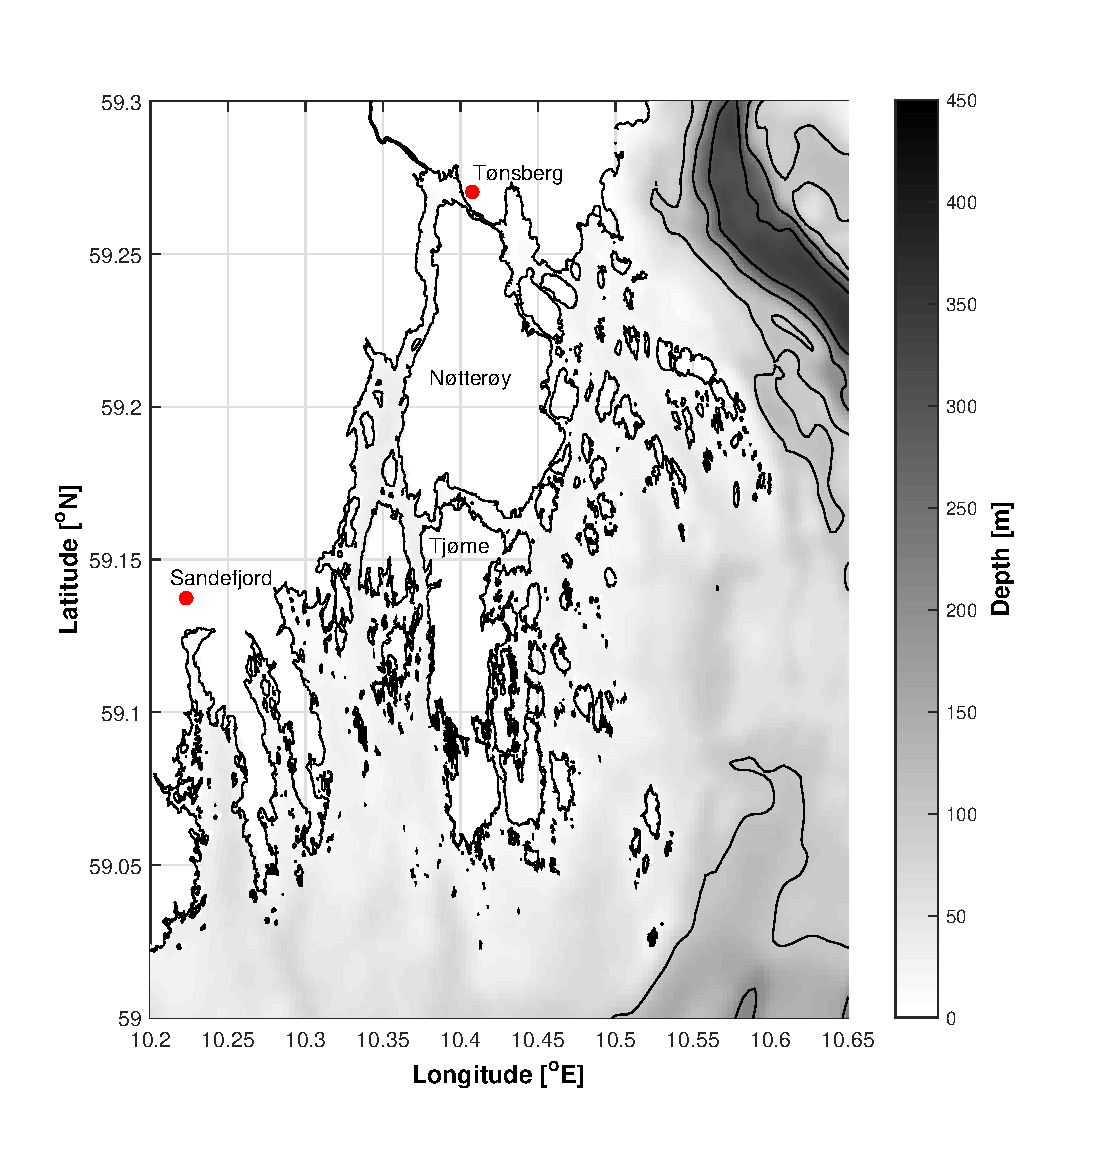
\includegraphics[height=6.8cm]{dyp_Tonsberg}}
   \rput[bl](7.5,0){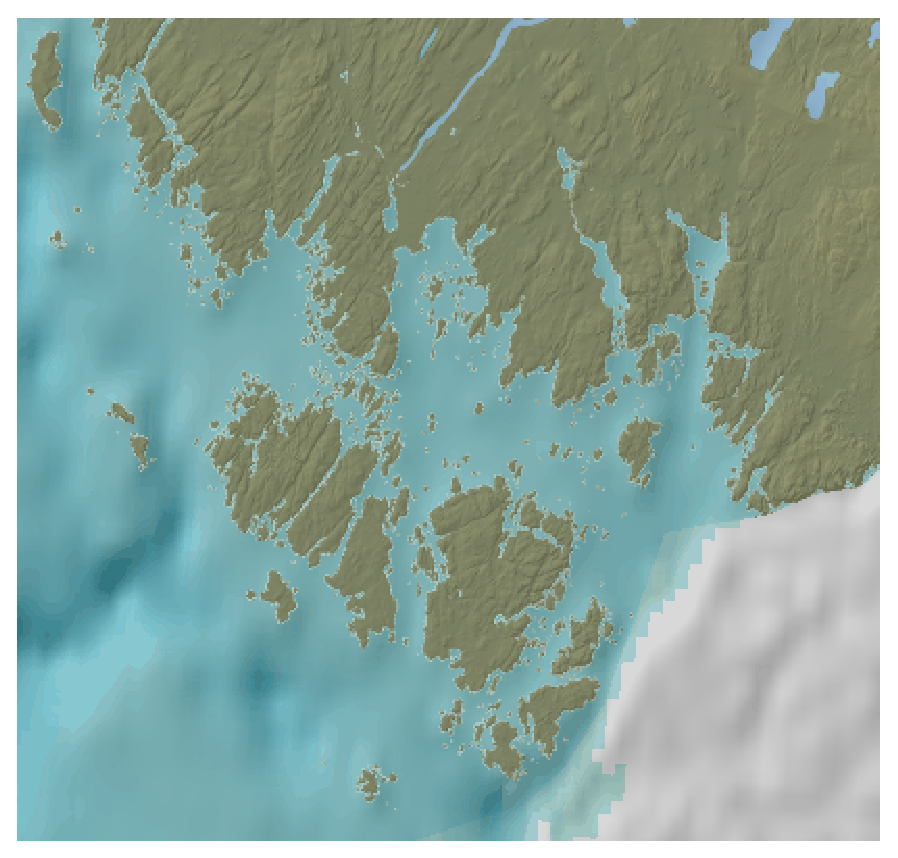
\includegraphics[height=6.8cm]{dyp_Hvaler}}
  \end{pspicture}
  \caption{\small The irregular coastline geometry and topography in the F{\ae}rder National Park (left-hand panel) and the Hvaler National Park (right-hand panel). Note the many islands, narrow straits and channels present in these areas of the Oslofjord.}
  \label{fig:ferder_hvaler}
 \end{center}
\end{figure}

